\documentclass[10pt]{beamer}
\usetheme[
%%% option passed to the outer theme
%    progressstyle=fixedCircCnt,   % fixedCircCnt, movingCircCnt (moving is deault)
  ]{Berlin}
  
% If you want to change the colors of the various elements in the theme, edit and uncomment the following lines

% Change the bar colors:
%\setbeamercolor{Feather}{fg=red!20,bg=red}

% Change the color of the structural elements:
%\setbeamercolor{structure}{fg=red}

% Change the frame title text color:
%\setbeamercolor{frametitle}{fg=blue}

% Change the normal text color background:
%\setbeamercolor{normal text}{fg=black,bg=gray!10}

%-------------------------------------------------------
% INCLUDE PACKAGES
%-------------------------------------------------------

\usepackage[utf8]{inputenc}
\usepackage[english]{babel}
\usepackage[T1]{fontenc}
\usepackage{amsmath}
\usepackage{helvet}
\usepackage{multirow}
\usepackage{graphicx}
\usepackage{comment}
\usepackage[absolute,overlay]{textpos}
\usepackage{tikz}
\usetikzlibrary{arrows,automata,positioning}
\usetikzlibrary{shapes.multipart}
\usetikzlibrary{decorations.markings}

%-------------------------------------------------------
% DEFFINING AND REDEFINING COMMANDS
%-------------------------------------------------------

% colored hyperlinks
%\renewcommand*{\Footnotemark}[1]{\NCC@makefnmark{#1}}
\newcommand{\chref}[2]{
  \href{#1}{{\usebeamercolor[bg]{Feather}#2}}
}
\newcommand{\tuple}[1]{{\langle #1 \rangle}}
\newcommand{\pre}{\mathsf{pre}}     % precondition
\newcommand{\eff}{\mathsf{eff}}     % effect
\newcommand{\cond}{\mathsf{cond}}   % conditional effect

\newcommand{\X}{\mathcal{X}}
\newcommand{\F}{\mathcal{F}}
\newcommand{\A}{\mathcal{A}}
\newcommand{\N}{\mathcal{N}}
\newcommand{\I}{\mathcal{I}}
\newcommand{\real}{\mathbb{R}}
\newcommand{\Dw}{\mathcal{D}}
\newcommand{\Xw}{\mathcal{X}}
\newcommand{\Aw}{\mathcal{A}}
\newcommand{\Rw}{\mathcal{R}}
\newcommand{\OO}{\mathcal{O}}
\newcommand{\tOO}{\wt{\OO}}
\newcommand{\II}[1]{\mathbb{I}{\left\{#1\right\}}}
\newcommand{\PP}[1]{\mathbb{P}\left[#1\right]}
\newcommand{\EE}[1]{\mathbb{E}\left[#1\right]}
\newcommand{\EEs}[2]{\mathbb{E}_{#2}\left[#1\right]}
\newcommand{\PPt}[1]{\mathbb{P}_t\left[#1\right]}
\newcommand{\EEt}[1]{\mathbb{E}_t\left[#1\right]}
\newcommand{\PPi}[1]{\mathbb{P}_i\left[#1\right]}
\newcommand{\EEi}[1]{\mathbb{E}_i\left[#1\right]}
\newcommand{\EEp}[1]{\mathbb{E}_{\pi,P}\left[#1\right]}
\newcommand{\EEcp}[2]{\mathbb{E}_{\pi,P}\left[\left.#1\right|#2\right]}
\newcommand{\PPc}[2]{\mathbb{P}\left[#1\left|#2\right.\right]}
\newcommand{\PPct}[2]{\mathbb{P}_t\left[#1\left|#2\right.\right]}
\newcommand{\PPcc}[2]{\mathbb{P}\left[\left.#1\right|#2\right]}
\newcommand{\PPcct}[2]{\mathbb{P}_t\left[\left.#1\right|#2\right]}
\newcommand{\PPcci}[2]{\mathbb{P}_i\left[\left.#1\right|#2\right]}
\newcommand{\EEc}[2]{\mathbb{E}\left[#1\left|#2\right.\right]}
\newcommand{\EEcc}[2]{\mathbb{E}\left[\left.#1\right|#2\right]}
\newcommand{\EEcs}[3]{\mathbb{E}_{#3}\left[\left.#1\right|#2\right]}
\newcommand{\EEcct}[2]{\mathbb{E}_t\left[\left.#1\right|#2\right]}
\newcommand{\EEcci}[2]{\mathbb{E}_i\left[\left.#1\right|#2\right]}
\renewcommand{\th}{\ensuremath{^{\mathrm{th}}}}
\def\argmin{\mathop{\mbox{ arg\,min}}}
\def\argmax{\mathop{\mbox{ arg\,max}}}
\newcommand{\ra}{\rightarrow}

\newcommand{\norm}[1]{\left\|#1\right\|}
\newcommand{\onenorm}[1]{\norm{#1}_1}
\newcommand{\infnorm}[1]{\norm{#1}_\infty}
\newcommand{\iprod}[2]{\left\langle#1,#2\right\rangle}
\newcommand{\ev}[1]{\left\{#1\right\}}
\newcommand{\pa}[1]{\left(#1\right)}
\newcommand{\bpa}[1]{\bigl(#1\bigr)}
\newcommand{\Bpa}[1]{\Bigl(#1\Bigr)}
\newcommand{\sign}{\mbox{sign}}
\newcommand{\wh}{\widehat}
\newcommand{\wt}{\widetilde}
\newcommand{\transpose}{^\top}

\newcommand{\loss}{\ell}
\newcommand{\hloss}{\wh{\loss}}
\newcommand{\hL}{\wh{L}}
\newcommand{\tZ}{\wt{Z}}
\newcommand{\reg}{\mathfrak{R}}
\newcommand{\hreg}{\widehat{\reg}}
\newcommand{\hr}{\wh{r}}
\newcommand{\hv}{\wh{v}}
\newcommand{\hq}{\wh{q}}
\newcommand{\hmu}{\wh{\mu}}
\newcommand{\hR}{\wh{R}}
\newcommand{\tmu}{\wt{\mu}}
\newcommand{\tN}{\wt{N}}
\newcommand{\RE}[2]{\mbox{RE}\left(\left.#1\right\|#2\right)}
\newcommand{\KL}[2]{\mbox{KL}\left(#1\middle\lVert#2\right)}
\newcommand{\DD}[3]{D_{#3}\left(#1\middle\lVert#2\right)}
\newcommand{\DDC}[2]{\DD{#1}{#2}{C}}
\newcommand{\DDS}[2]{\DD{#1}{#2}{S}}

\newcommand{\trho}{\wt{\rho}}

\definecolor{gold}{rgb}{1,0.75,0}
\definecolor{darkred}{rgb}{0.75,0,0}
\setbeamercolor*{goldc}{fg=black,bg=gold}
\definecolor{darkpurp}{rgb}{0.4,0.2,0.4}
\setbeamercolor*{purpc}{fg=white,bg=darkpurp}
\setbeamercolor*{redc}{fg=white,bg=darkred}
\newcommand{\hG}[1]{\large \textcolor{darkred}{#1}}

\newcommand{\redd}[1]{\textcolor{darkred}{#1}}
\newcommand{\goldd}[1]{\textcolor{gold}{#1}}

\definecolor{ballblue}{rgb}{0.0, 0.53, 0.74}
\definecolor{lightgray}{rgb}{0.85, 0.85, 0.85}

%-------------------------------------------------------
% INFORMATION IN THE TITLE PAGE
%-------------------------------------------------------

\title[] % [] is optional - is placed on the bottom of the sidebar on every slide
{ % is placed on the title page
      \textbf{Machine Learning}
}

\author[Jonsson \& G\'omez]
{      Anders Jonsson \& Vicen\c{c} G\'omez \\
\vspace*{0.5cm}
Master in Intelligence Interactive Systems\\
2020-21\\
\vspace*{0.5cm}
Lecture 3\\
Bias-Variance Tradeoff and Overfitting
%      {\ttfamily bagchi.bhaskar@cse.iitkgp.ernet.in}
}

\date{}

\AtBeginSection[]
{
   \begin{frame}
       \frametitle{Content}
       \tableofcontents[currentsection]
   \end{frame}
}

%-------------------------------------------------------
% THE BODY OF THE PRESENTATION
%-------------------------------------------------------

\begin{document}

%-------------------------------------------------------
% THE TITLEPAGE
%-------------------------------------------------------

\begin{frame}[plain,noframenumbering] % the plain option removes the header from the title page, noframenumbering removes the numbering of this frame only
  \titlepage % call the title page information from above
\end{frame}

\begin{frame}{Content}{}
\tableofcontents
\end{frame}

\section{Generalization and VC dimension}

\begin{frame}
  \frametitle{True loss vs. training loss}
  \begin{itemize}
	\item {\color{purple} True loss} or {\color{purple} risk} $L_{\mathcal{D},f}(h)$ measures the mistakes of $h$ on the entire {\color{blue} domain set $\mathcal{X}$} (with distribution $\mathcal{D}$ and labelling function $f$)
	\item {\color{red} Training loss} or {\color{red} empirical risk} $L_S(h)$ measures the mistakes of $h$ on the {\color{cyan} training set $S=((x_1,y_1),\ldots,(x_m,y_m))$}
	\item Want $h$ with small $L_{\mathcal{D},f}(h)$, but can only measure $L_S(h)$
	\[L_{\mathcal{D},f}(h) = L_S(h) + {\color{red} (L_{\mathcal{D},f}(h) - L_S(h))}\]
	\item Generalization: minimize $L_{\mathcal{D},f}(h) - L_S(h)$
  \end{itemize}
\end{frame}

\begin{frame}
  \frametitle{Generalization properties}
  \begin{itemize}
	\item How well does $L_S(h)$ approximate $L_{\mathcal{D},f}(h)$?
	\item Hoeffding's inequality for a single, fixed hypothesis $h$:
	\[
	\mathbb{P}\left[|L_S(h) - L_{\mathcal{D},f}(h)| > \epsilon\right] \leq 2 e^{-2m\epsilon^2}
	\]
	\item Hypothesis $h_S$ that minimizes the empirical risk:
	\[
	\mathbb{P}\left[|L_S(h_S) - L_{\mathcal{D},f}(h_S)| > \epsilon\right] \leq 2 {\color{red} |\mathcal{H}|}e^{-2m\epsilon^2}
	\]
  \end{itemize}
\end{frame}

\begin{frame}
  \frametitle{VC dimension}
  \begin{itemize}
	\item Problem: $\mathcal{H}$ is often an {\color{red} infinite set} $\Rightarrow |\mathcal{H}|$ is {\color{red} unbounded}
	\item Vapnik-Chervonenkis (VC) dimension $D_{VC}$: {\color{green} effective size} of $\mathcal{H}$
	\item Hypothesis $h_S$ that minimizes the empirical risk:
	\[
	\mathbb{P}\left[|L_S(h_S) - L_{\mathcal{D},f}(h_S)| > \epsilon\right] \leq 2 {\color{red} D_{VC}}e^{-2m\epsilon^2}
	\]
  \end{itemize}
\end{frame}

\begin{frame}
  \frametitle{VC dimension}
  \begin{center}
  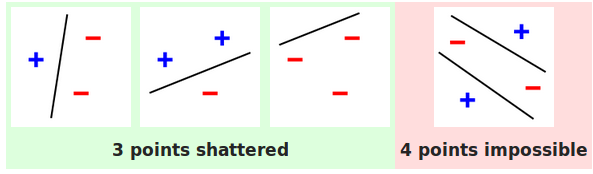
\includegraphics[height=3cm]{images/vcdim.png}
  \end{center}
\end{frame}

\begin{frame}
  \frametitle{Model complexity}
  \begin{itemize}
	\item For linear models, $|\mathcal{H}|=\infty$ but {\color{green} $D_{VC}=d+1$}!
	\item {\color{red} Model complexity}: number of model parameters (e.g.~weights)
	\item $D_{VC}$ is often proportional to the model complexity
	\item A {\color{blue} more complex model} is {\color{purple} less likely to generalize well}!
	\item {\color{cyan} Alternative formulation} of Hoeffding's inequality:
	\[
	L_{\mathcal{D},f}(h_S) \leq L_S(h_S) + \Omega(m,{\color{red} D_{VC}})
	\]
  \end{itemize}
\end{frame}

\begin{frame}
  \frametitle{Learning curves}
  \begin{center}
  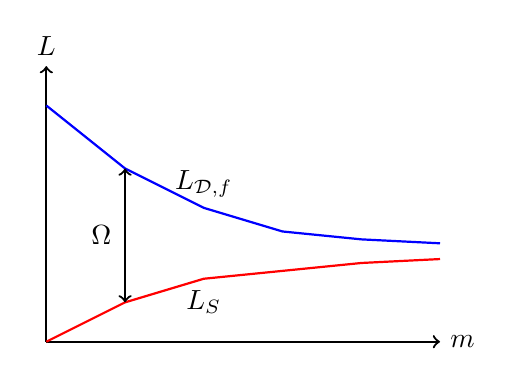
\begin{tikzpicture}
  \draw[thick,->] (0,0) -- (5,0) node[right]{$m$};
  \draw[thick,->] (0,0) -- (0,3.5) node[above]{$L$};
  \draw[thick,red] plot [smooth] (0,0) -- (1,0.5) -- (2,0.8) -- (3,0.9) -- (4,1) -- (5,1.05);
  \draw[thick,blue] plot [smooth] (0,3) -- (1,2.2) -- (2,1.7) -- (3,1.4) -- (4,1.3) -- (5,1.25);
  \node at (2,0.5) {$L_S$};
  \node at (2,2) {$L_{\mathcal{D},f}$};
  \draw[thick,<->] (1,0.5) -- (1,2.2);
  \node at (0.7,1.35) {$\Omega$};
  \end{tikzpicture}
  \end{center}
  \begin{itemize}
	\item The training loss usually {\color{red} increases} as a function of $m$
	\item The true loss usually {\color{blue} decreases} as a function of $m$
	\item Equivalently, $\Omega(m,D_{VC})$ {\color{green} decreases} as a function of $m$
  \end{itemize}
\end{frame}

\begin{frame}
  \frametitle{No Free Lunch theorem}
  \begin{itemize}
	\item Let $\mathcal{A}$ be any binary classification algorithm on domain set $\mathcal{X}$
	\item Let $m\leq|\mathcal{X}|/2$ be the size of the training set $S$
  \end{itemize}
  \pause
  \begin{theorem}
	There exist $\mathcal{D}$ and $f$ such that with probability at least $1/7$ on the choice of $S$, it holds that $L_{\mathcal{D},f}(\mathcal{A}(S)) \geq 1/8$
  \end{theorem}
  \pause
	{\color{red} No algorithm} does well on all learning problems!
\end{frame}

\section{Bias and variance}

\begin{frame}
  \frametitle{Bias}
  \begin{center}
  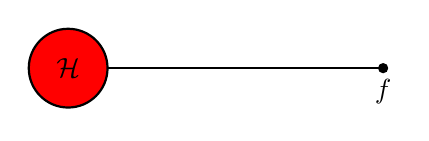
\begin{tikzpicture}
  \draw[thick,fill=red] (-2,0) circle (0.5cm);
  \node at (-2,0) {$\mathcal{H}$};
  \draw[thick] (-1.5,0) -- (2,0);
  \draw[thick,fill=black] (2,0) circle (0.05cm);
  \node at (2,-0.3) {$f$};
  \end{tikzpicture}
  \end{center}
  \begin{itemize}
	\item It is essential to {\color{blue} restrict} the class $\mathcal{H}$ of hypothesis functions
	\item However, too much restriction {\color{red} prevents us} from approximating $f$!
	\item {\color{purple} Bias}: how ``far'' the labelling function $f$ is from the class $\mathcal{H}$
  \end{itemize}
\end{frame}

\begin{frame}
  \frametitle{Variance}
  \begin{center}
  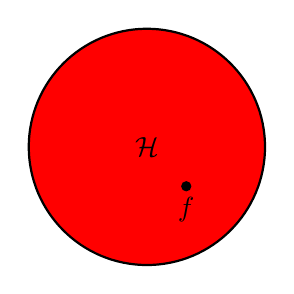
\begin{tikzpicture}
  \draw[thick,fill=red] (0,0) circle (1.5cm);
  \node at (0,0) {$\mathcal{H}$};
  \draw[thick,fill=black] (0.5,-0.5) circle (0.05cm);
  \node at (0.5,-0.8) {$f$};
  \end{tikzpicture}
  \end{center}
  \begin{itemize}
	\item The larger the hypothesis class, the more likely it is to include $f$
	\item However, this makes it more difficult to zoom in on the correct $f$
	\item {\color{purple} Variance}: how far the ERM hypothesis $h_S$ is from $f$ on average
  \end{itemize}
\end{frame}

\begin{frame}
  \frametitle{Learning curves}
  \begin{center}
  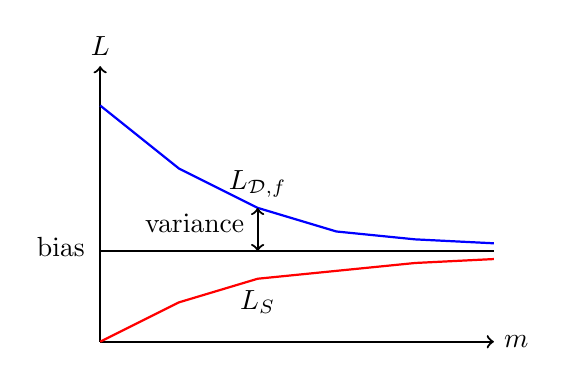
\begin{tikzpicture}
  \draw[thick,->] (0,0) -- (5,0) node[right]{$m$};
  \draw[thick,->] (0,0) -- (0,3.5) node[above]{$L$};
  \draw[thick,red] plot [smooth] (0,0) -- (1,0.5) -- (2,0.8) -- (3,0.9) -- (4,1) -- (5,1.05);
  \draw[thick,blue] plot [smooth] (0,3) -- (1,2.2) -- (2,1.7) -- (3,1.4) -- (4,1.3) -- (5,1.25);
  \node at (2,0.5) {$L_S$};
  \node at (2,2) {$L_{\mathcal{D},f}$};
  \draw[thick] (0,1.15) -- (5,1.15);
  \node at (-0.5,1.2) {bias};
  \draw[thick,<->] (2,1.15) -- (2,1.7);
  \node at (1.2,1.5) {variance};
  \end{tikzpicture}
  \end{center}
  \begin{itemize}
	\item {\color{red} Bias} determines the theoretical limit of $L_{\mathcal{D},f}$
	\item {\color{blue} Variance} determines how far $L_{\mathcal{D},f}$ is from this limit
	\item Variance {\color{green} decreases} as a function of $m$
  \end{itemize}
\end{frame}

\begin{frame}
  \frametitle{Bias-variance tradeoff}
  \begin{center}
  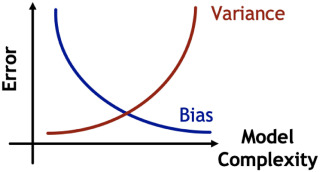
\includegraphics[height=3cm]{images/model.jpg}
  \end{center}
  \begin{itemize}
	\item Less complex model $\Rightarrow$ more bias
	\item More complex model $\Rightarrow$ more variance
	\item {\color{red} Tradeoff}: impossible to achieve $0$ bias and $0$ variance
  \end{itemize}
\end{frame}

\begin{frame}
  \frametitle{Bias-variance characterization}
  Regression task, squared error, ERM hypothesis $h_S$:
  \[
  \begin{cases}
  \begin{aligned}
  \action<+->{\mathbb{E}_{S\sim\mathcal{D},f} &\{ L_{\mathcal{D},f}(h_S) \} = \mathbb{E}_{S\sim\mathcal{D},f} \{ \mathbb{E}_{x\sim\mathcal{D}} \{ (h_S(x) - f(x))^2 \} \} \\}
  \action<+->{ &= \mathbb{E}_{x\sim\mathcal{D}} \{ \mathbb{E}_{S\sim\mathcal{D},f} \{ (h_S(x) - f(x))^2 \} \} \\}
  \action<+->{ &= \mathbb{E}_{x\sim\mathcal{D}} \{ \mathbb{E}_{S\sim\mathcal{D},f} \{ (h_S(x) - \overline{h}(x) + \overline{h}(x) - f(x))^2 \} \} \\}
  \action<+->{ &= \mathbb{E}_{x\sim\mathcal{D}} \{ \mathbb{E}_{S\sim\mathcal{D},f} \{ (h_S(x) - \overline{h}(x))^2 + (\overline{h}(x) - f(x))^2 \\}
  \action<+->{ & \hspace*{2.7cm} + 2({\color{red} h_S(x) - \overline{h}(x)})(\overline{h}(x) - f(x)) \} \} \\}
  \action<+->{ &= \mathbb{E}_{x\sim\mathcal{D}} \{ \mathbb{E}_{S\sim\mathcal{D},f} \{ (h_S(x) - \overline{h}(x))^2 \} + (\overline{h}(x) - f(x))^2 + {\color{red} 0} \} \\}
  \action<+->{ &= \mathbb{E}_{x\sim\mathcal{D}} \{ \hspace*{1.0cm} {\color{blue} variance}(x) \hspace*{1.0cm} + \hspace*{.6cm} {\color{red} bias}(x) \hspace*{.6cm} \} \\}
  \action<+->{ &= {\color{blue} variance} + {\color{red} bias} }
  \end{aligned}
  \end{cases}
  \]
  \pause
  $\overline{h}(x) = \mathbb{E}_{S\sim\mathcal{D},f} \{ h_S(x) \}$: {\color{purple} average} ERM hypothesis on input $x$
\end{frame}

\begin{frame}
  \frametitle{Example}
  \begin{center}
  \begin{tikzpicture}
  \draw[thick,->] (0,0) -- (5,0) node[right]{$x$};
  \draw[thick,->] (0,0) -- (0,3) node[left]{$y$};
  \draw[thick, blue] (0,1.5) sin (1.25,0.8);
  \draw[thick, blue] (2.5,1.5) sin (1.25,0.8);
  \draw[thick, blue] (2.5,1.5) sin (3.75,2.2);
  \draw[thick, blue] (5,1.5) sin (3.75,2.2);
  \end{tikzpicture}
  \end{center}
  \begin{itemize}
  \item Assume that $f$ is a sine curve
  \item $\mathcal{H}_0$: {\color{green} constant} hypotheses
  \item $\mathcal{H}_1$: {\color{red} linear} hypotheses
  \item $m=2$: only sample 2 data points
  \item Which hypothesis class is better?
  \end{itemize}
\end{frame}

\begin{frame}
  \frametitle{Comparison}
  \begin{center}
  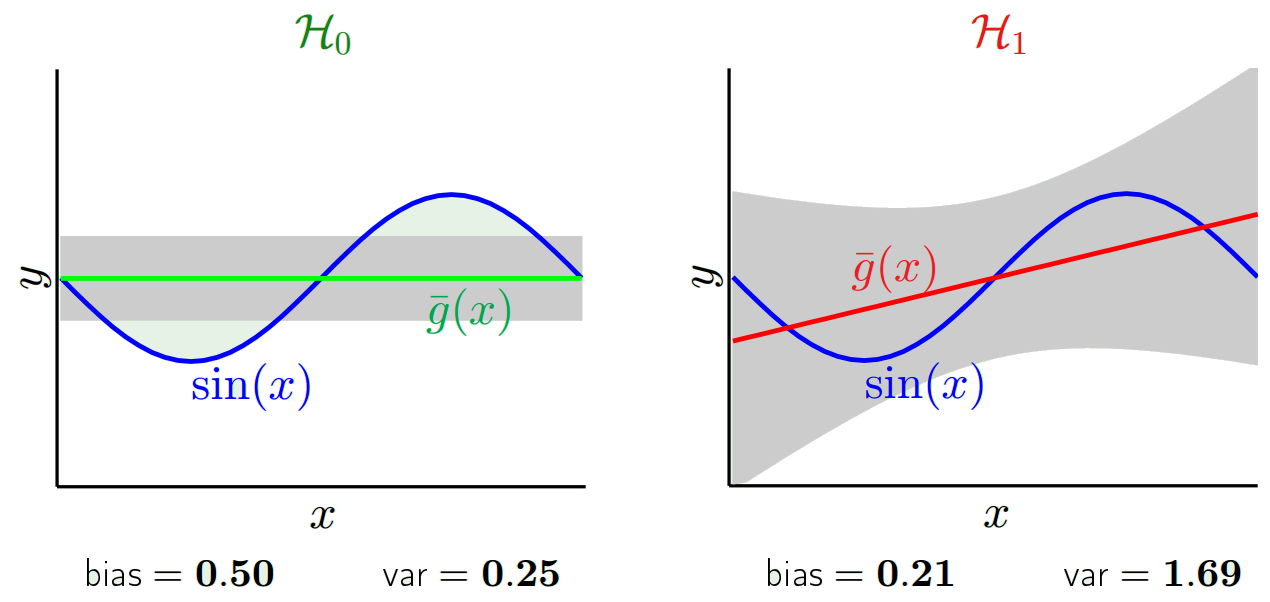
\includegraphics[height=5cm]{images/sine.png}
  \end{center}
  $\overline{g}(x)=\overline{h}(x)$: {\color{purple} average} ERM hypothesis on input $x$
\end{frame}

\section{Overfitting}

\begin{frame}
  \frametitle{Overfitting}
  \begin{center}
  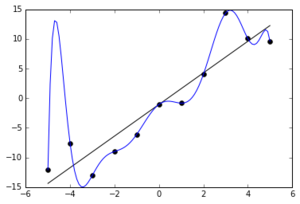
\includegraphics[height=3cm]{images/overfit.png}
  \end{center}
  \begin{itemize}
	\item We can often make the training loss smaller using a more complex model
	\item {\color{red} Overfitting}: sacrifice true loss for smaller training loss
  \end{itemize}
\end{frame}

\begin{frame}
  \frametitle{Learning curves}
  \begin{center}
  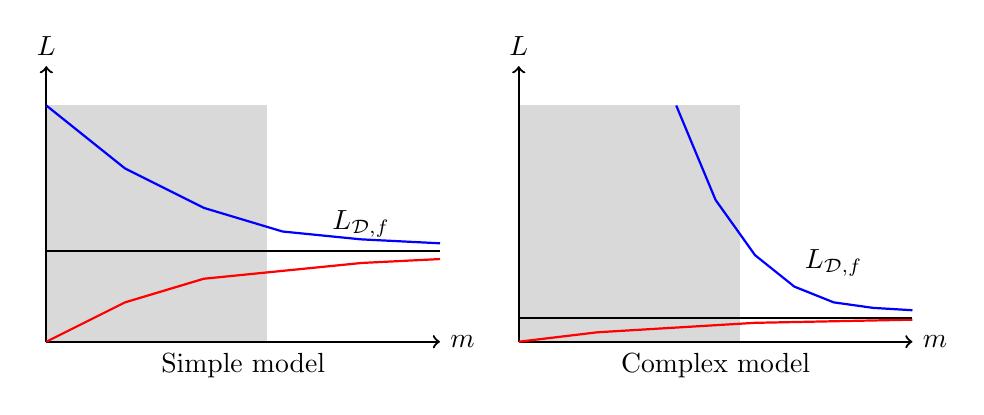
\begin{tikzpicture}
  \draw[fill=lightgray,lightgray] (-6,0) rectangle (-3.2,3);
  \draw[thick,->] (-6,0) -- (-1,0) node[right]{$m$};
  \draw[thick,->] (-6,0) -- (-6,3.5) node[above]{$L$};
  \draw[thick,red] plot [smooth] (-6,0) -- (-5,0.5) -- (-4,0.8) -- (-3,0.9) -- (-2,1) -- (-1,1.05);
  \draw[thick,blue] plot [smooth] (-6,3) -- (-5,2.2) -- (-4,1.7) -- (-3,1.4) -- (-2,1.3) -- (-1,1.25);
  \node at (-2,1.5) {$L_{\mathcal{D},f}$};
  \draw[thick] (-6,1.15) -- (-1,1.15);
  \node at (-3.5,-0.3) {Simple model};

  \draw[fill=lightgray,lightgray] (0,0) rectangle (2.8,3);
  \draw[thick,->] (0,0) -- (5,0) node[right]{$m$};
  \draw[thick,->] (0,0) -- (0,3.5) node[above]{$L$};
  \draw[thick,red] plot [smooth] (0,0) -- (1,0.12) -- (2,0.18) -- (3,0.24) -- (4,0.26) -- (5,0.28);
  \draw[thick,blue] plot [smooth] (2,3) -- (2.5,1.8) -- (3,1.1) -- (3.5,0.7) -- (4,0.5) -- (4.5,0.43) -- (5,0.4);
  \node at (4,1) {$L_{\mathcal{D},f}$};
  \draw[thick] (0,0.3) -- (5,0.3);
  \node at (2.5,-0.3) {Complex model};
  \end{tikzpicture}
  \end{center}
  \begin{itemize}
	\item Higher model complexity $\Rightarrow$ {\color{red} smaller training loss $L_S(h)$}
	\item Poor generalization properties $\Rightarrow$ {\color{blue} larger true loss $L_{\mathcal{D},f}(h)$}
  \end{itemize}
\end{frame}

\begin{frame}
  \frametitle{Overfitting and bias-variance tradeoff}
  \begin{center}
  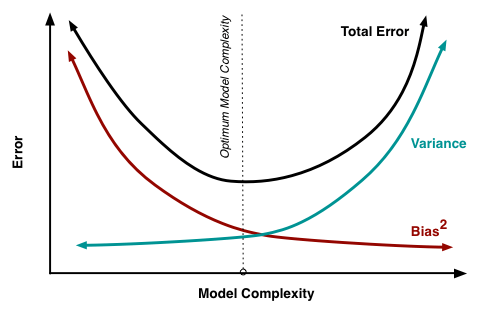
\includegraphics[height=5cm]{images/overfitting.png}
  \end{center}
  \begin{itemize}
	\item There exists a theoretical {\color{blue} optimum model complexity}
	\item Increasing the model complexity more causes the loss to blow up
	\item {\color{green} In practice}: better to start with simpler models!
  \end{itemize}
\end{frame}

\begin{frame}
  \frametitle{Regularization}
  \begin{itemize}
	\item Technique that helps overcome the problem of overfitting
	\item {\color{red} Linear models}: introduce constraints on the weight vector $w$
	\item {\color{blue} Constrained optimization}:
	\[\min L_S(w) \;\;\;\; \mathrm{s.t.} \sum_{i=0}^d w_i^2\leq C\]
	\item Difficult (NP-hard) to optimize
  \end{itemize}
\end{frame}

\begin{frame}
  \frametitle{Regularization}
  \begin{itemize}
	\item {\color{red} Alternative definition}: add extra term to loss function:
	\[L_{aug}(w)=L_S(w)+\frac \lambda m w^\top w\]
	\item $\sum w_i^2$: {\color{blue} L2-norm, weighted decay}
	\item $\sum |w_i|$: {\color{green} L1-norm, sparsity}
	\item {\color{cyan} Difficulty}: no analytical way to select $\lambda$
	\item {\color{green} Linear regression}: $w_{reg}=(X^\top X+\lambda I)^{-1}X^\top y$
  \end{itemize}
\end{frame}

\begin{frame}
  \frametitle{Regularization}
  \begin{center}
  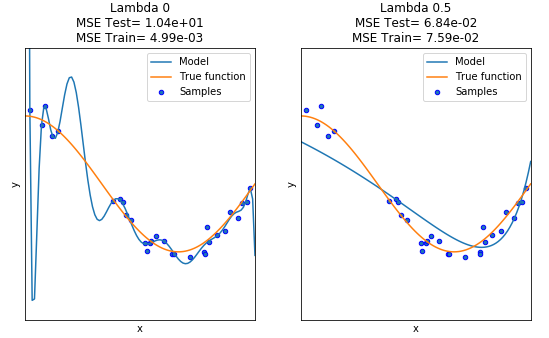
\includegraphics[height=5.5cm]{images/reg.png}
  \end{center}
\end{frame}

\begin{frame}
  \frametitle{Validation}
  \begin{itemize}
	\item Alternative to overcome overfitting
	\item Used for {\color{red} model selection}: learning algorithm, non-linear transform, regularizer, parameters, etc.
	\item Due to overfitting, selecting by $L_S(h)$ is not always a good idea!
	\item {\color{blue} Validation}: approximate $L_{\mathcal{D},f}(h)$ better (but still optimistic!)
  \end{itemize}
\end{frame}

\begin{frame}
  \frametitle{Validation}
  \begin{itemize}
	\item In addition to $S$, assume {\color{red} validation set} $V=((x_1,y_1),\ldots,(x_n,y_n))$
	\item Also assume that $V$ is sampled independently of $S$
	\item {\color{blue} Validation loss} $L_V(h)$ is a much better estimate of $L_{\mathcal{D},f}(h)$!
	\item {\color{green} In practice}: divide dataset into training set and validation set
  \end{itemize}
\end{frame}

\begin{frame}
  \frametitle{Model selection}
  \begin{itemize}
	\item Train $M$ alternative models on training set $S$
	\item Compute validation error $L_V(h_S)$ on each resulting hypothesis
	\item Select model with smallest validation error, retrain on entire $S\cup V$
  \end{itemize}
  \begin{center}
  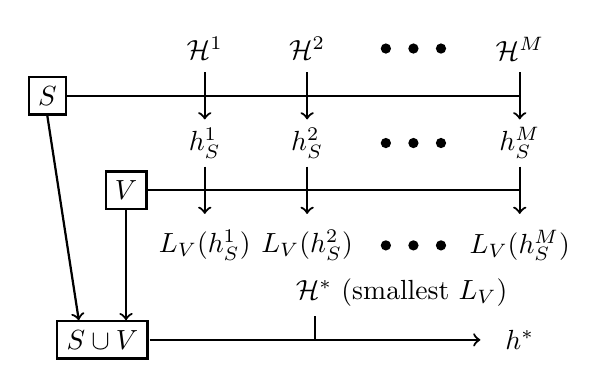
\begin{tikzpicture}
  \node at (1,3.6) {$\mathcal{H}^1$};
  \node at (2.3,3.6) {$\mathcal{H}^2$};
  \draw[thick,fill=black] (3.3,3.6) circle (0.05cm);
  \draw[thick,fill=black] (3.65,3.6) circle (0.05cm);
  \draw[thick,fill=black] (4,3.6) circle (0.05cm);
  \node at (5,3.6) {$\mathcal{H}^M$};

  \node[thick,draw] at (-1,3) {$S$};
  \draw[thick] (-0.75,3) -- (5,3);
  \draw[thick,->] (1,3.3) -- (1,2.7);
  \draw[thick,->] (2.3,3.3) -- (2.3,2.7);
  \draw[thick,->] (5,3.3) -- (5,2.7);

  \node at (1,2.4) {$h_S^1$};
  \node at (2.3,2.4) {$h_S^2$};
  \draw[thick,fill=black] (3.3,2.4) circle (0.05cm);
  \draw[thick,fill=black] (3.65,2.4) circle (0.05cm);
  \draw[thick,fill=black] (4,2.4) circle (0.05cm);
  \node at (5,2.4) {$h_S^M$};

  \node[thick,draw] at (0,1.8) {$V$};
  \draw[thick] (0.25,1.8) -- (5,1.8);
  \draw[thick,->] (1,2.1) -- (1,1.5);
  \draw[thick,->] (2.3,2.1) -- (2.3,1.5);
  \draw[thick,->] (5,2.1) -- (5,1.5);

  \node at (1,1.1) {$L_V(h_S^1)$};
  \node at (2.3,1.1) {$L_V(h_S^2)$};
  \draw[thick,fill=black] (3.3,1.1) circle (0.05cm);
  \draw[thick,fill=black] (3.65,1.1) circle (0.05cm);
  \draw[thick,fill=black] (4,1.1) circle (0.05cm);
  \node at (5,1.1) {$L_V(h_S^M)$};

  \node[thick,draw] at (-0.3,-0.1) {$S\cup V$};
  \draw[thick,->] (-1,2.75) -- (-0.6,0.15);
  \draw[thick,->] (0,1.55) -- (0,0.15);
  \draw[thick,->] (0.3,-0.1) -- (4.5,-0.1);

  \node at (3.5,0.5) {$\mathcal{H}^*$ (smallest $L_V$)};
  \node at (5,-0.1) {$h^*$};
  \draw[thick] (2.4,0.2) -- (2.4,-0.1);
  \end{tikzpicture}
  \end{center}
\end{frame}

\begin{frame}
  \frametitle{Cross-validation}
  \begin{center}
  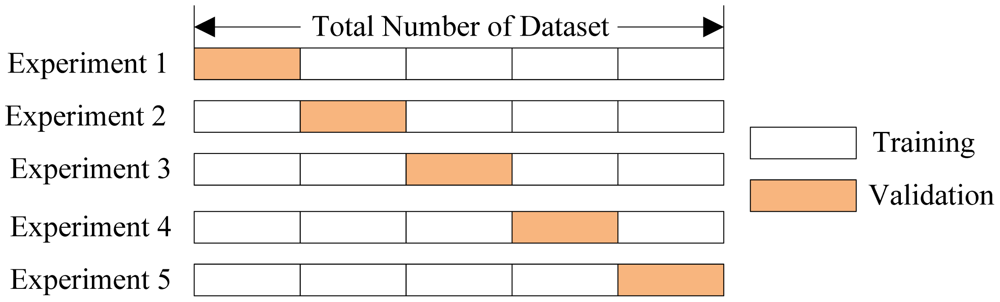
\includegraphics[height=2.5cm]{images/cross.png}
  \end{center}
  \begin{itemize}
	\item Partition $S$ into $k$ subsets $S_1,\ldots,S_k$, each of size $m/k$
	\item In each experiment, train on $S\setminus S_i$ and validate on $S_i$
	\item {\color{red} Cross-validation loss} is the average across experiments:
	\[L_{cv}(\theta)=\frac 1 k \sum_{i=1}^k L_{S_i}(h_i)\]
	\item {\color{green} In practice}: $k=5$ or $k=10$ are usually good choices
  \end{itemize}
\end{frame}

\begin{frame}
  \frametitle{Cross-validation}
  \begin{center}
  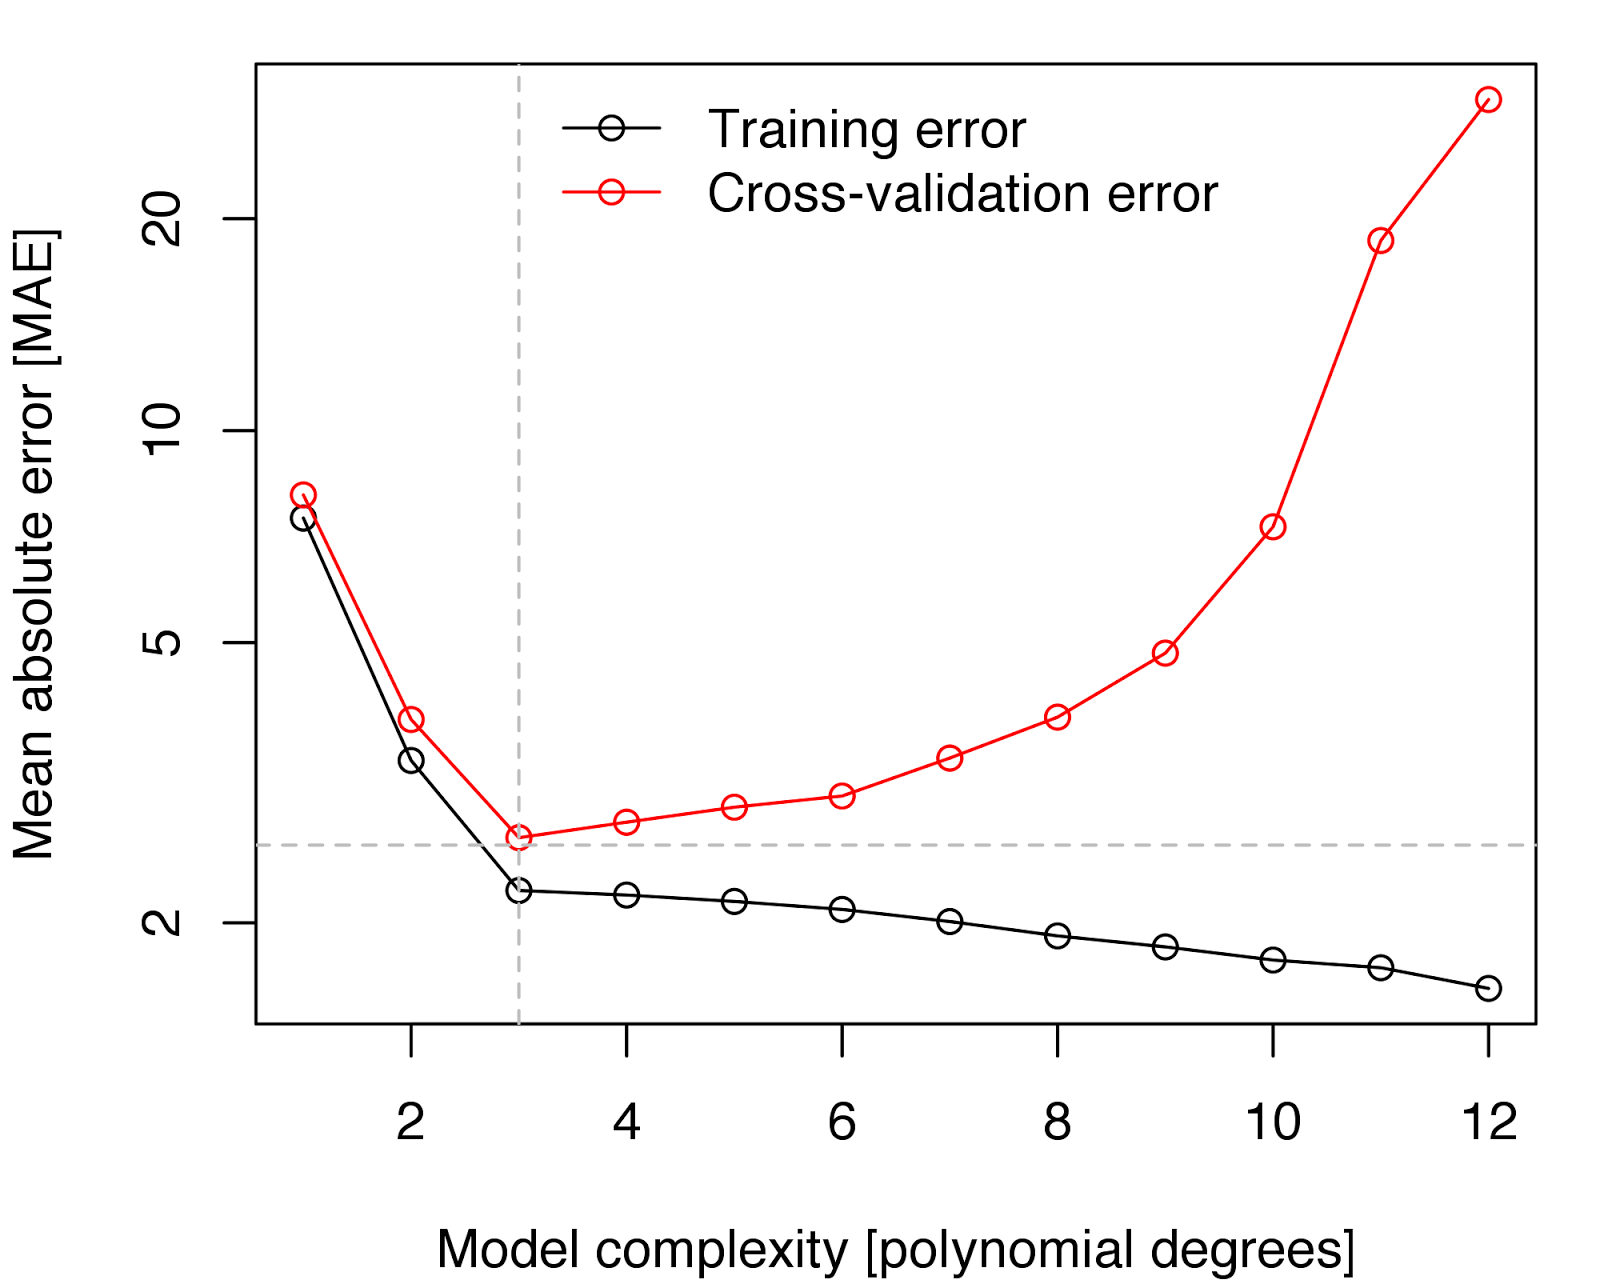
\includegraphics[height=6.5cm]{images/crosserr.png}
  \end{center}
\end{frame}

\end{document}

